%!TEX program = xelatex
%!TEX TS-program = xelatex
%!TEX encoding = UTF-8 Unicode
\documentclass[a4paper]{uestcreport}
% =============================================
% Part 0 Edit the info
% =============================================
\major{翻译专业}
\name{张三}
\title{本科实验报告}
\stuid{2xxxxxxxxxxxx}
\college{外国语学院}
\date{\zhtoday}
\lab{寝室}
\course{数据库原理及应用}
\instructor{李四}
% \grades{}
% \expname{}
% \exptype{}
% \partner{}

\begin{document}
% =============================================
% Part 1 Header
% =============================================
\makecover
% \makeheader

% =============================================
% Part 2 Main document
% =============================================
\begin{center}
    \Large
    实验一:创建数据库
\end{center}
\thispagestyle{fancy}
\section{实验学时}
4学时

\section{实验内容和目的}
创建数据库Stud,该数据库包含五个表,名称如下:
\begin{itemize}
    \item 系别代码表——dep
    \item 教师表——teacher
    \item 学生表——student
    \item 课程表——course
    \item 选课表——sc
\end{itemize}

通过练习实验操作,掌握数据库和表的创建,熟悉数据库的常见数据类型。

\section{实验原理}
数据库的创建、删除:
\begin{lstlisting}[language=SQL]
    DROP DATABASE [databasename];
    CREATE DATABASE [databasename];
\end{lstlisting}

创建表:
\begin{lstlisting}[language=SQL]
    CREATE TABLE [数据库名.][用户名.]<基表名>(
        <列名1><列类型><列约束>,
        <列名2><列类型><列约束>,
        ...
        <列名n><列类型><列约束>;
    );
\end{lstlisting}

\section{实验器材}
数据库服务器环境:Microsoft SQL SERVER 2008

VSCode搭配MSSQL插件执行SQL语句。

\section{实验步骤}
\subsection{创建数据库}
创建名为stud的数据库:
\begin{lstlisting}[language=SQL]
    -- Drop existing database of the same name
    DROP DATABASE stud;
    -- Create Database stud
    CREATE DATABASE stud;
\end{lstlisting}

\subsection{创建系别代码表dep}
\begin{lstlisting}[language=SQL]
    -- Create Table dep
    CREATE TABLE dep
    (
        depid VARCHAR(10) PRIMARY KEY,
        depname VARCHAR(20) NOT NULL
    );
\end{lstlisting}

\subsection{创建教师表teacher}
\begin{lstlisting}[language=SQL]
    -- Create Table teacher
    CREATE TABLE teacher
    (
        tid VARCHAR(8) PRIMARY KEY,
        tname VARCHAR(8) NOT NULL,
        title VARCHAR(10),
        depid VARCHAR(8)
    );
\end{lstlisting}

\subsection{创建学生表student}
\begin{lstlisting}[language=SQL]
    -- Create Table student
    CREATE TABLE student
    (
        studid VARCHAR(11) PRIMARY KEY,
        sname VARCHAR(8) NOT NULL,
        sex CHAR(2) NOT NULL,
        depid VARCHAR(8),
        birthd DATE,
        semail VARCHAR(20),
        homeaddr VARCHAR(40)
    );
\end{lstlisting}

\subsection{创建课程表course}
\begin{lstlisting}[language=SQL]
    -- Create Table course
    CREATE TABLE course
    (
        cid VARCHAR(8) PRIMARY KEY,
        cname VARCHAR(30) NOT NULL,
        credits NUMERIC(3, 2) NOT NULL,
    );
\end{lstlisting}

\subsection{创建选课表sc}
\begin{lstlisting}[language=SQL]
    -- Create Table sc
    CREATE TABLE sc
    (
        sstudid VARCHAR(11) NOT NULL,
        cid VARCHAR(8) NOT NULL,
        tid VARCHAR(8) NOT NULL,
        score INTEGER
    );
\end{lstlisting}

设置sstudid和cid为sc的主键(Primary Key):
\begin{lstlisting}[language=SQL]
    -- Add PRIMARY KEYS
    ALTER TABLE sc
        ADD CONSTRAINT pk_sc PRIMARY KEY (sstudid, cid);
\end{lstlisting}

\section{实验数据及结果分析}
成功创建stud数据库与dep、teacher、student、course和sc五个表。

五个表各自结构如下:
\begin{table}[!h]
    \centering
    \caption{系别代码表 dep}\label{tab:depTable}%添加标题 设置标签
    \begin{tabular}{|c|c|c|c|c|}
        \hline
        字段名称     & 字段类型 & 字段大小/格式 & 是否可为空 & 约束条件 \\
        \hline
        系代码 depid & varchar  & 8             & 否         & PK       \\
        \hline
        系名 depname & varchar  & 20            & 否         & Not null \\
        \hline
    \end{tabular}
    %\caption{这是一张三线表}\label{tab:aStrangeTable}  标题放在这里也是可以的
\end{table}

\begin{table}[!h]
    \centering
    \caption{教师表 teacher}\label{tab:teacherTable}%添加标题 设置标签
    \begin{tabular}{|c|c|c|c|c|}
        \hline
        字段名称     & 字段类型 & 字段大小/格式 & 是否可为空 & 约束条件 \\
        \hline
        教师号 tid   & varchar  & 8             & 否         & PK       \\
        \hline
        教师名 tname & varchar  & 8             & 否         & Not null \\
        \hline
        职称 title   & varchar  & 10            & 是         &          \\
        \hline
        所属院系编号 & varchar  & 8             & 是         &          \\
        \hline
    \end{tabular}
    %\caption{这是一张三线表}\label{tab:aStrangeTable}  标题放在这里也是可以的
\end{table}

\begin{table}[!h]
    \centering
    \caption{学生表 student}\label{tab:studentTable}%添加标题 设置标签
    \begin{tabular}{|c|c|c|c|c|}
        \hline
        字段名称          & 字段类型 & 字段大小/格式 & 是否可为空 & 约束条件 \\
        \hline
        学号 studid       & varchar  & 8             & 否         & PK       \\
        \hline
        学生名 sname      & varchar  & 8             & 否         & Not null \\
        \hline
        性别 sex          & char     & 2             & 是         &          \\
        \hline
        院系编号 depid    & varchar  & 8             & 是         &          \\
        \hline
        出生年月 birthd   & date     &               & 是         &          \\
        \hline
        邮箱 semail       & varchar  & 20            & 是         &          \\
        \hline
        家庭地址 homeaddr & varchar  & 40            & 是         &          \\
        \hline
    \end{tabular}
    %\caption{这是一张三线表}\label{tab:aStrangeTable}  标题放在这里也是可以的
\end{table}

\begin{table}[!h]
    \centering
    \caption{课程表 course}\label{tab:courseTable}%添加标题 设置标签
    \begin{tabular}{|c|c|c|c|c|}
        \hline
        字段名称     & 字段类型 & 字段大小/格式 & 是否可为空 & 约束条件 \\
        \hline
        课程号 cid   & varchar  & 8             & 否         & PK       \\
        \hline
        课程名 cname & varchar  & 30            & 否         & Not null \\
        \hline
        学分 credits & numeric  & 3(小数位1)    & 否         & Not null \\
        \hline
    \end{tabular}
    %\caption{这是一张三线表}\label{tab:aStrangeTable}  标题放在这里也是可以的
\end{table}

\begin{table}[!h]
    \centering
    \caption{选课表sc}\label{tab:scTable}%添加标题 设置标签
    \begin{tabular}{|c|c|c|c|c|}
        \hline
        字段名称     & 字段类型 & 字段大小/格式 & 是否可为空 & 约束条件 \\
        \hline
        学号 sstudid & varchar  & 11            & 否         & PK       \\
        \hline
        课程号 cid   & varchar  & 8             & 否         & PK       \\
        \hline
        教师号 tid   & varchar  & 8             & 否         & Not null \\
        \hline
        成绩 score   & integer  &               & 是         &          \\
        \hline
    \end{tabular}
    %\caption{这是一张三线表}\label{tab:aStrangeTable}  标题放在这里也是可以的
\end{table}

\newpage
\section{实验结论、心得体会和改进建议}
创建表时应注意表各属性的信息。

应熟练掌握数据库的创建、销毁以及表的创建和数据库的基本数据类型。

\newpage
\begin{center}
    \Large
    实验二:数据库的完整性
\end{center}

\setcounter{section}{0}
\section{实验学时}
4学时

\section{实验内容和目的}
通过设置表的检查约束、外键约束体和数据库完整性的含义,约束条件下数据修改操作的限制,以及实现修改操作的技巧。

\section{实验原理}
\subsection{基本表的修改(添加、删除约束):}
\begin{lstlisting}[language=SQL]
    ALTER TABLE <基表名>
        ADD CONSTRAINT <约束名> <约束定义>;
    ALTER TABLE <基表名>
        DROP CONSTRAINT <约束名>;
\end{lstlisting}

\subsection{外键约束:}
对外码的取值限定称为外键(FOREIGN KEY)约束。设$F$是基本关系$R$的一个或一组属性,但不是关系$R$的码。如果$F$与基本关系$S$的主码
$K$相对应,则称$F$是基本关系$R$的外码。$R$中每个元组在$F$上的值必须为:或取空值,或者等于$S$中某个元组的主码值。

外键约束的声明有两种方式:
\begin{enumerate}
    \item 外码为单属性,则可在属性名称、类型名称之后,用REFERENCES指出被参照的关系、属性,形式为:
          \begin{lstlisting}[language=SQL]
        REFERENCES <被参照表表名> (<属性名>)
    \end{lstlisting}
    \item 在CREATE TABLE定义语句的属性列描述之后,将一个或多个属性列声明为外码,形式为:
          \begin{lstlisting}[language=SQL]
        FOREIGN KEY (<属性名>) REFERENCES <被参照表表名> (<属性名>)
    \end{lstlisting}
\end{enumerate}

\subsection{字符串比较:}
当两个字符串里的字符序列完全相同时成两个字符串相等。使用如$<$或$>$等比较运算符对字符串作比较运算时,实际上比较的
是他们的字母表顺序。SQL提供的另外以中国字符串比较方式:
\begin{lstlisting}[language=SQL]
    属性列 [NOT] LIKE 字符串常量
\end{lstlisting}

这里的字符串常量不仅指普通的字符,还可以包括通配符。使用LIKE运算符和通配符可以实现模糊查询。

通配符如下:
\begin{itemize}
    \item \_(下划线):匹配任意一个字符。
    \item \%(百分号):匹配任意长度的字符。
    \item $[]$:查询一定范围的数据,用于指定一定范围内的任何单个字符,包括两端数据。
    \item $[\^{}]$:查询本来不属于指定范围的,如([a-f])或集合([abcdef])的任何单个字符。
\end{itemize}

\section{实验步骤}
\subsection{设置约束条件}
\begin{enumerate}
    \item 设置教师表,学生表中的院系字段(depid)的外键约束:\\
          \begin{lstlisting}[language=SQL]
        ALTER TABLE teacher
            ADD CONSTRAINT fk_teacher FOREIGN KEY(depid) REFERENCES dep(depid);
        ALTER TABLE student
            ADD CONSTRAINT fk_student FOREIGN KEY(depid) REFERENCES dep(depid);
    \end{lstlisting}
    \item 设置选课表的三个外键约束(学号,课程号,教师号):\\
          \begin{lstlisting}[language=SQL]
        ALTER TABLE sc
            ADD CONSTRAINT fk_sstudid FOREIGN KEY(sstudid) REFERENCES student(studid);
        ALTER TABLE sc
            ADD CONSTRAINT fk_cid FOREIGN KEY(cid) REFERENCES course(cid);
        ALTER TABLE sc
            ADD CONSTRAINT fk_tid FOREIGN KEY(tid) REFERENCES teacher(tid);
    \end{lstlisting}
    \item 设置选课表中成绩字段的取值范围是0到100:\\
          \begin{lstlisting}[language=SQL]
        ALTER TABLE sc
            ADD CONSTRAINT ck_score CHECK (score>=0 AND score<=100);
    \end{lstlisting}
    \item 设置学生表中性别字段的取值位“男”或“女”:\\
          \begin{lstlisting}[language=SQL]
        ALTER TABLE student
            ADD CONSTRAINT ck_sex CHECK (sex IN ('男', '女'));
    \end{lstlisting}
    \item 设置学生表电子邮件字段的取值必须包含@符号:\\
          \begin{lstlisting}[language=SQL]
        ALTER TABLE student
            ADD CONSTRAINT ck_email CHECK (semail LIKE '%@%');
    \end{lstlisting}
\end{enumerate}

\subsection{使用INSERT语句向数据库添加数据:}
\begin{lstlisting}[language=SQL]
    -- Insert Datas
    INSERT INTO dep
    VALUES
        ('601', '计算机科学与工程'),
        ('602', '软件工程'),
        ('603', '信息安全');

    INSERT INTO teacher
    VALUES
        ('T01', '教师1', '教授', '601'),
        ('T02', '教师2', '工程师', '601'),
        ...
        ('T06', '教师6', '高工', '603');

    INSERT INTO student
    VALUES
        ('00', 'Bill', '男', '1988-02-12', 'bill@ms.net', NULL, '601'),
        ('101', '陈刚', '男', '1995-10-02', 's101@stu.net', '1栋25号', '601'),
        ...
        ('164', '周敏', '男', '1996-03-12', 's164@stu.net', '1栋41号', '602');

    INSERT INTO course
    VALUES
        ('6001', '计算机组成原理', '3'),
        ('6002', '操作系统', '3'),
        ('6003', '数据结构', '3'),
        ...
        ('6011', '数据库应用开发', '2');

    INSERT INTO SC
    VALUES
        ('101', '6001', 'T01', NULL),
        ('101', '6002', 'T01', NULL),
        ('101', '6003', 'T01', NULL),
        ...
        ('164', '6011', 'T01', '52');
\end{lstlisting}

\section{实验数据及结果分析}
使用SELECT语句可验证数据已成功插入。

最终stud数据库内五个表可视化关系如下图:
\begin{figure}[!htbp]
    \centering
    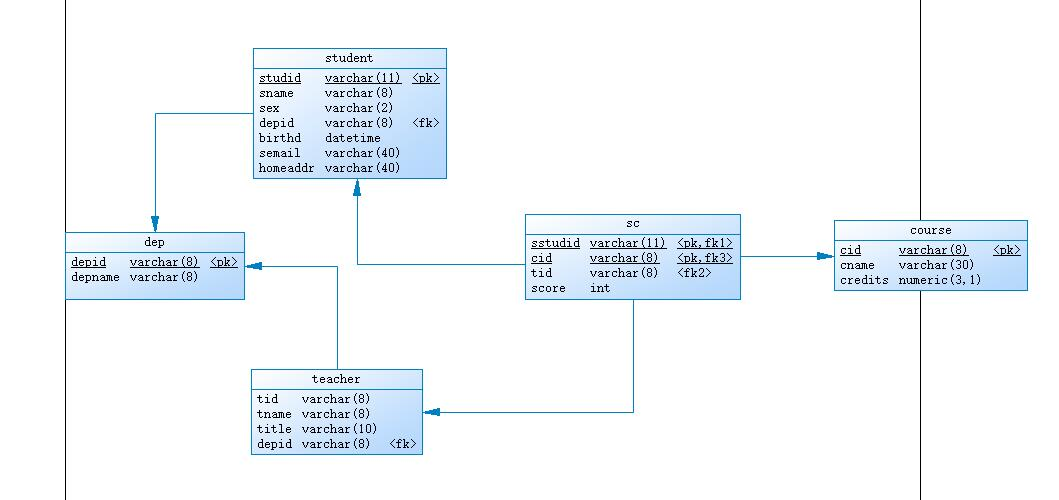
\includegraphics[width=0.8\linewidth]{relation.jpg}
    \caption{表可视化关系图}
\end{figure}

\section{实验结论、心得体会和改进建议}
熟练掌握数据库的完整性、约束条件、结构化查询语言相关知识。

\newpage
\begin{center}
    \Large
    实验三:数据的修改
\end{center}

\setcounter{section}{0}
\section{实验学时}
4学时

\section{实验内容和目的}
练习UPDATE、DELETE命令的使用,实现对数据的修改和删除,同时体会主键、外键及约束条件对修改操作的限制。

\section{实验原理}
\subsection{数据更新:}
可使用UPDATE语句对数据进行更新,其语句的一般格式为:
\begin{lstlisting}[language=SQL]
    UPDATE <基表名>
    SET <属性列名>=<表达式>[,<属性列名>=<表达式>...]
    [WHERE <行选择条件>]
\end{lstlisting}

\subsection{数据删除:}
可使用DELETE语句删除某些元组,其语句的一般格式为:
\begin{lstlisting}[language=SQL]
    DELETE FROM <基表名>
    [WHERE <行选择条件>]
\end{lstlisting}

\section{实验步骤}
\begin{enumerate}
    \item 将院系表中,原院系名“IS”改为“Information”:
          \begin{lstlisting}[language=SQL]
        INSERT INTO dep
        VALUES
            ('604', 'IS');
        UPDATE dep SET depname='Information' WHERE depid='604';
    \end{lstlisting}
    \item 在选课表中,删除计算机科学与工程系学生选修2号课程的记录:
          \begin{lstlisting}[language=SQL]
        DELETE sc WHERE cid='6002' AND sstudid IN (SELECT sstudid
            FROM student JOIN dep ON dep.depid=student.depid
            WHERE dep.depname='601');
    \end{lstlisting}
    \item 在选课表中,删除软件工程系学生选课1号课程的记录:
          \begin{lstlisting}[language=SQL]
        DELETE sc WHERE cid='6001' AND sstudid IN (SELECT sstudid
            FROM student JOIN dep ON dep.depid=student.depid
            WHERE dep.depname='软件工程');
    \end{lstlisting}
    \item 将学号为“601”的学生的学号改为“20060601”,且同时更改该学生所有的选课信息,保证使用新学号后选购的课程不丢失:
          \begin{lstlisting}[language=SQL]
        INSERT INTO student
            (studid,sname,sex,birthd,semail,homeaddr,depid)
        SELECT '20060601', sname, sex, birthd, semail, homeaddr, depid
        FROM student
        WHERE studid='101';
        UPDATE sc SET sstudid='20060601' WHERE sstudid='101';
        DELETE student WHERE studid='101';
    \end{lstlisting}
    \item 使用UPDATE语句登记考试成绩:
          \begin{lstlisting}[language=SQL]
        UPDATE sc SET score=99 WHERE sstudid='102' AND cid='6011';
    \end{lstlisting}
\end{enumerate}

\section{实验数据及结果分析}
使用SELECT语句可验证数据已成功更新。

\section{实验结论、心得体会和改进建议}
熟练掌握结构化查询语言。

\newpage
\begin{center}
    \Large
    实验四:简单查询、多表查询
\end{center}

\setcounter{section}{0}
\section{实验学时}
4学时

\section{实验内容和目的}
练习使用SELECT查询语句,设置查询条件,实现单表查询。

练习使用SELECT语句,从多个表中查询数据,表的连接的使用以及设置连接条件,区分连接条件和查询条件在
目的和功能上的区别。

\section{实验原理}
\subsection{连接查询}
\subsubsection{内连接}
内连接是在不明确指明连接类型的情况下默认的连接类型,它要求参与连接运算的表满足给定的连接条件。内连接
可以通过WHERE语句和JOIN子句两种方式实现。
\begin{itemize}
    \item WHERE语句连接:
          \begin{lstlisting}[language=SQL]
        FROM 表1,表2 WHERE <连接条件>
    \end{lstlisting}
    \item JOIN子句:
          \begin{lstlisting}[language=SQL]
        FROM 表1 [INNER] JOIN 表2 ON <连接条件>
    \end{lstlisting}
\end{itemize}

\subsubsection{外连接}
外连接可以从一张表或者同时从两张表中获得不匹配的行,这样的操作,就叫做外连接。

外连接分为左外连接、右外连接和全外连接三种:
\begin{itemize}
    \item 左外连接。\\
          左外连接的结果包括了LEFT OUTER JOIN子句中指定的左表的所有行,而不仅是连接列所匹配的行。常见格式为:
          \begin{lstlisting}[language=SQL]
        FROM 表1 LEFT OUTER JOIN 表2 ON <连接条件>
    \end{lstlisting}
    \item 右外连接。\\
          右外连接是左外连接的反向连接,将返回右表的所有行。常见格式为:
          \begin{lstlisting}[language=SQL]
        FROM 表1 RIGHT OUTER JOIN 表2 ON <连接条件>
    \end{lstlisting}
    \item 全外连接。\\
          完整外部连接返回左表和右表中的所有行。常见格式为:
          \begin{lstlisting}[language=SQL]
        FROM 表1 FULL OUTER JOIN 表2 ON <连接条件>
    \end{lstlisting}
\end{itemize}

\section{实验步骤}
\begin{enumerate}
    \item 查询年龄在20-30之间的学生姓名:
          \begin{lstlisting}[language=SQL]
        SELECT studid 学生编号, sname 学生姓名, year(getdate())-year(birthd) 年龄
        FROM student
        WHERE year(getdate())-year(birthd)>=20 AND year(getdate())-year(birthd)<=30;
    \end{lstlisting}
    \item 查询所有副教授的信息:
          \begin{lstlisting}[language=SQL]
        SELECT tid 教师编号, tname 教师姓名, depid 院系编号
        FROM teacher
        WHERE title='副教授';
    \end{lstlisting}
    \item 查询姓“孙”的学生的学号、姓名和邮件地址:
          \begin{lstlisting}[language=SQL]
        SELECT studid 学号, sname 姓名, semail 邮件地址
        FROM student
        WHERE sname LIKE '孙%';
    \end{lstlisting}
    \item 查询所有成绩(成绩不为空)的学生学号和课程号:
          \begin{lstlisting}[language=SQL]
        SELECT sstudid 学生学号, cid 课程号
        FROM sc
        WHERE score IS NOT NULL;
    \end{lstlisting}
    \item 查询选修了6003号课程成绩在60分以下的所有学生的学号、姓名、课程名及课程成绩:
          \begin{lstlisting}[language=SQL]
        SELECT sc.sstudid 学号, student.sname 姓名, course.cname 课程名称, sc.score 课程成绩
        FROM sc JOIN student ON sc.sstudid = student.studid JOIN course ON sc.cid = course.cid
        WHERE sc.score<60 AND sc.cid='6003';
    \end{lstlisting}
    \item 查询选修了“数据库原理”的学生学号和姓名及教师姓名:
          \begin{lstlisting}[language=SQL]
        SELECT sc.sstudid 学号, student.sname 学生姓名, teacher.tname 教师名称
        FROM sc JOIN student ON sc.sstudid = student.studid JOIN teacher ON sc.tid=teacher.tid JOIN course ON sc.cid = course.cid
        WHERE course.cname='数据库原理';
    \end{lstlisting}
\end{enumerate}

\section{实验数据及结果分析}
使用SELECT语句可验证返回结果正确。

\section{实验结论、心得体会和改进建议}
熟练掌握结构化查询语言、表的连接和关系运算相关知识。

\newpage
\begin{center}
    \Large
    实验五:分组统计查询
\end{center}

\setcounter{section}{0}
\section{实验学时}
4学时

\section{实验内容和目的}
练习使用聚集函数COUNT(), MAX(), MIN(), AVG()等在SQL命令中实现统计功能。

使用GROUP BY子句实现分组查询,以及聚集函数在分组查询中的应用。

体会分组查询的功能特点。

\section{实验原理}
\subsection{聚集函数}
SQL提供的聚集函数包括SUM(求和函数)、MAX(最大值函数)、MIN(最小值函数)、AVG(平均值函数)和COUNT(计数
函数)等,聚集函数的名称及功能如下表:
\begin{table}[!h]
    \centering
    \caption{聚集函数的名称及功能}\label{tab:funcsTable}%添加标题 设置标签
    \begin{tabular}{|c|c|}
        \hline
        函数名称 & 函数功能                           \\
        \hline
        SUM      & 返回选取结果集合中所有值的和       \\
        \hline
        COUNT    & 返回选取结果集合中所有记录行的数目 \\
        \hline
        MAX      & 返回选取结果集中所有值的最大值     \\
        \hline
        MIN      & 返回选取结果集中所有值的最小值     \\
        \hline
        AVG      & 返回选取结果集中所有值的平均值     \\
        \hline
    \end{tabular}
    %\caption{这是一张三线表}\label{tab:aStrangeTable}  标题放在这里也是可以的
\end{table}

\subsection{GROUP BY子句}
GROUP BY子句将某一列数据的值进行分类。其子句基本结构为:
\begin{lstlisting}[language=SQL]
    [GROUP BY <分组依据列>]
\end{lstlisting}

\subsection{HAVING子句}
HAVING子句指定组或聚合的搜索条件。若HAVING子句不予GROUP BY子句搭配,则作用与WHERE子句相同。其子句基本
结构为:
\begin{lstlisting}[language=SQL]
    [HAVING <search_condition>]
\end{lstlisting}

\section{实验步骤}
\begin{enumerate}
    \item 查询选修数据库课程的人数:
          \begin{lstlisting}[language=SQL]
        SELECT COUNT(*)
        FROM sc JOIN course ON sc.cid=course.cid
        WHERE course.cname='数据库原理';
    \end{lstlisting}
    \item 求每个学生选课的门数,显示学号和选课门数:
          \begin{lstlisting}[language=SQL]
        SELECT sc.sstudid 学号, COUNT(cid) 选课门数
        FROM sc
        GROUP BY sc.sstudid;
    \end{lstlisting}
    \item 求每个学生选课的总学分数,显示学号和学分:
          \begin{lstlisting}[language=SQL]
        SELECT sc.sstudid 学号, SUM(course.credits) 总学分数
        FROM sc JOIN course ON sc.cid=course.cid
        GROUP BY sc.sstudid;
    \end{lstlisting}
    \item 查询选修数据库并且成绩在60分以上的人数:
          \begin{lstlisting}[language=SQL]
        SELECT COUNT(*) 总人数
        FROM sc JOIN course ON course.cid=sc.cid
        WHERE course.cname='数据库原理' AND sc.score>60;
    \end{lstlisting}
    \item 求每门课程的选课人数、最高分、最低分和平均分,并显示课程名:
          \begin{lstlisting}[language=SQL]
        SELECT course.cname 课程名, COUNT(sc.sstudid) 选课人数, MAX(sc.score) 最高分, MIN(sc.score) 最低分, AVG(sc.score) 平均分
        FROM sc JOIN course ON sc.cid=course.cid
        GROUP BY course.cname;
    \end{lstlisting}
    \item 求选修了5门以上课程的学生姓名和邮件地址:
          \begin{lstlisting}[language=SQL]
        SELECT student.sname 学生姓名, student.semail 邮件地址
        FROM sc JOIN student ON sc.sstudid=student.studid
        GROUP BY student.sname,student.semail
        HAVING count(*)>5;
    \end{lstlisting}
\end{enumerate}

\section{实验数据及结果分析}
使用SELECT语句可验证返回结果正确。

\section{实验结论、心得体会和改进建议}
熟练掌握结构化查询语言、分组查询、集函数相关知识。

\newpage
\begin{center}
    \Large
    实验六:集合操作、子查询
\end{center}

\setcounter{section}{0}
\section{实验学时}
4学时

\section{实验内容和目的}
练习IN、EXISTS、NOT EXISTS运算在WHERE子句中的应用。

练习静态集合和由SELECT命令产生的动态结果集运算。

\section{实验原理}
\subsection{集合运算}
SQL Server提供的集合运算符由UNION、EXCEPT和INTERSECT。其中,UNION运算符实现集合并运算,EXCEPT运算符
实现集合差运算,INTERSECT运算符实现集合交运算。

\subsection{嵌套查询(子查询)}
查询的条件子句含有SELECT查询子句,则称这样的查询为嵌套查询;外层的查询称为主查询(或父查询),内层的SELECT
查询子句称为子查询。

SQL Server提供了IN、NOT IN等运算符用于集合成员的测试。

\section{实验步骤}
\begin{enumerate}
    \item 查询其他系中比信息系(depid=\'601\')某一学生年龄小的学生姓名和年龄:
          \begin{lstlisting}[language=SQL]
        SELECT sname 学生姓名, YEAR(GETDATE())-YEAR(birthd) 年龄
        FROM student
        WHERE YEAR(GETDATE())-YEAR(birthd)<ANY(SELECT YEAR(GETDATE())-YEAR(birthd)
        FROM student
        WHERE depid='601');
    \end{lstlisting}
    \item 查询没有选修任何课程的学生姓名、所在院系及邮件地址:
          \begin{lstlisting}[language=SQL]
        SELECT sname 学生姓名, depid 所在院系, semail 邮件地址
        FROM student
        WHERE studid NOT IN (SELECT DISTINCT studid
        FROM sc);
    \end{lstlisting}
    \item 查询选修了全部课程的学生姓名:
          \begin{lstlisting}[language=SQL]
        SELECT sname 学生名称
        FROM student
        WHERE NOT EXISTS (
        SELECT cid
        FROM course
        WHERE cid NOT IN (SELECT cid
        FROM sc
        WHERE sc.sstudid=student.studid));
    \end{lstlisting}
    \item 查询既选修了6003号课程,又选修了6004号课程的学生学号:
          \begin{lstlisting}[language=SQL]
        SELECT sstudid 学生编号
        FROM sc
        WHERE sc.cid='6003' AND sstudid IN (SELECT sstudid
            FROM sc
            WHERE sc.cid='6004');
    \end{lstlisting}
    \item 查询既选修了6003号课程,由选修了6004号课程的学生姓名:
          \begin{lstlisting}[language=SQL]
        SELECT sname 学生姓名
        FROM sc JOIN student ON sstudid = student.studid
        WHERE sc.cid='6003' AND sstudid IN (SELECT sstudid
            FROM sc
            WHERE sc.cid='6004');
    \end{lstlisting}
\end{enumerate}

\section{实验数据及结果分析}
使用SELECT语句可验证返回结果正确。

\section{实验结论、心得体会和改进建议}
熟练掌握结构化查询语言、集合运算、子查询相关知识。

\newpage
\begin{center}
    \Large
    实验七:数据库建模
\end{center}

\setcounter{section}{0}
\section{实验学时}
4学时

\section{实验内容和目的}
学习数据库建模工具Power Designer最基本的使用方法,使用物理数据模型(PDM),以图形化界面方式创建表确定各表之间的关系。

通过物理模型生成创建数据库的脚本。

\section{实验原理}
\subsection{物理数据模型PDM}
PDM叙述数据库的物理实现。

藉由PDM,考虑真实的物理实现的细节。它进入帐户两个软件或数据储藏结构之内。能修正PDM适合你的表现或物理约束。

主要目的是把CDM中建立的现实世界模型生成特定的DBMS脚本,产生数据库中保存信息的储存结构,保证数据在数据库中的
完整性和一致性。

PDM是适合于系统设计阶段的工具。

\section{实验步骤}
\subsection{生成PDM以图形化界面创建表及确定各表之间的关系:}
\begin{enumerate}
    \item 创建PDM\_Stud物理数据模型。
          \begin{figure}[!htbp]
              \centering
              \includegraphics[width=0.8\linewidth]{PDM.jpg}
              \caption{PDM\_Stud}
          \end{figure}
          \newpage
    \item 分别创建dep、teacher、course、sc和student表。
          \begin{figure}[!htbp]
              \centering
              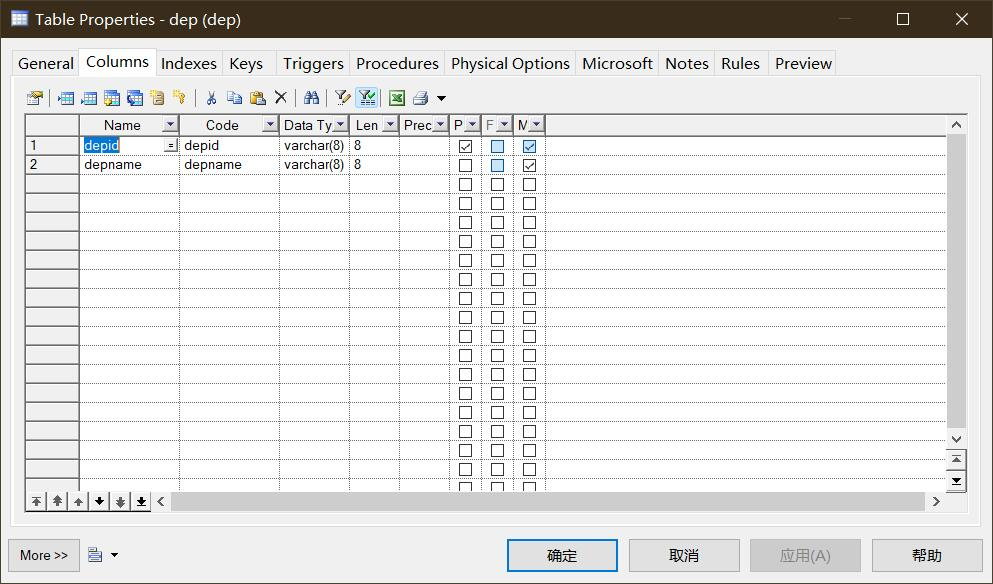
\includegraphics[width=0.8\linewidth]{dep.jpg}
              \caption{dep}
          \end{figure}
          \begin{figure}[!htbp]
              \centering
              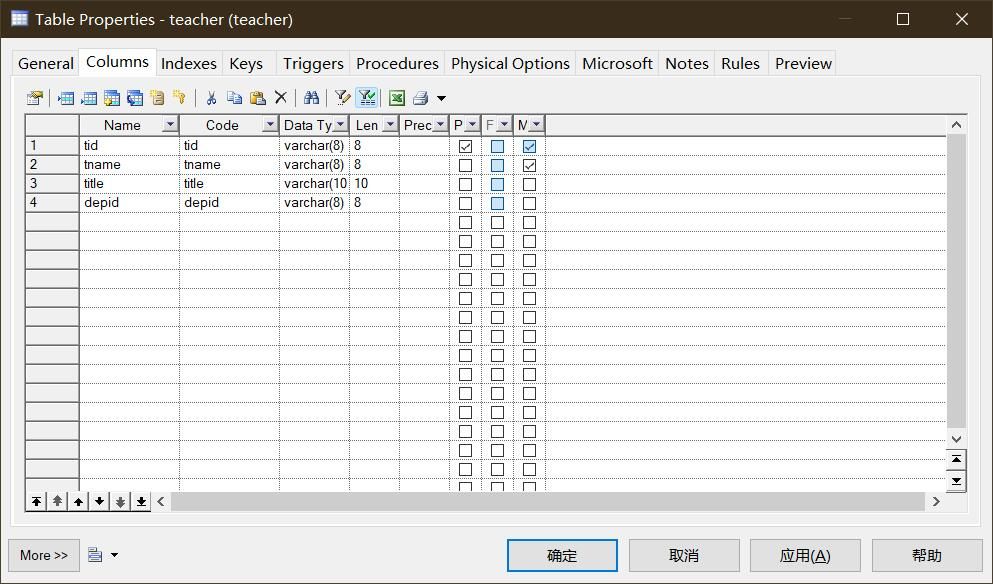
\includegraphics[width=0.8\linewidth]{teacher.jpg}
              \caption{teacher}
          \end{figure}
          \begin{figure}[!htbp]
              \centering
              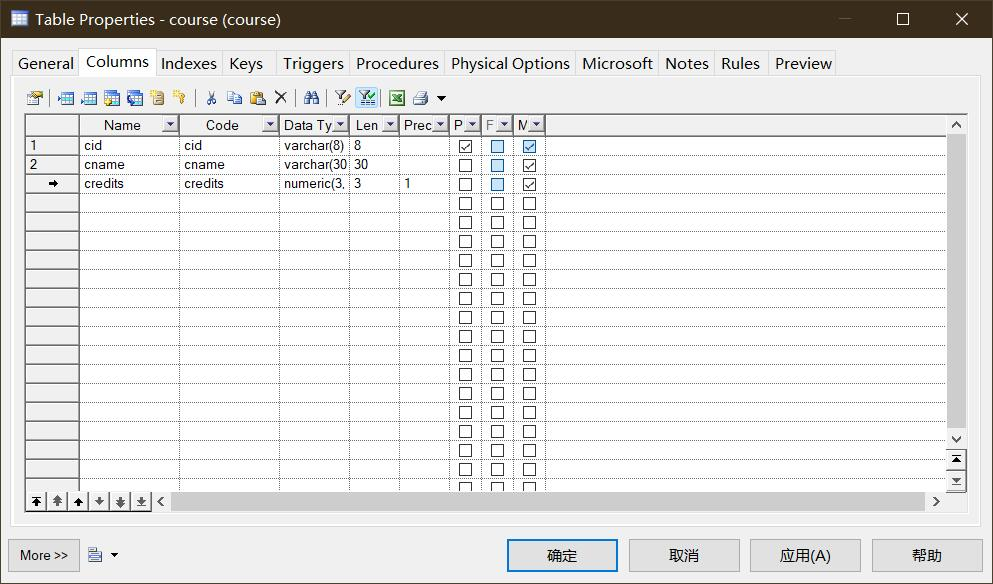
\includegraphics[width=0.8\linewidth]{course.jpg}
              \caption{course}
          \end{figure}
          \begin{figure}[!htbp]
              \centering
              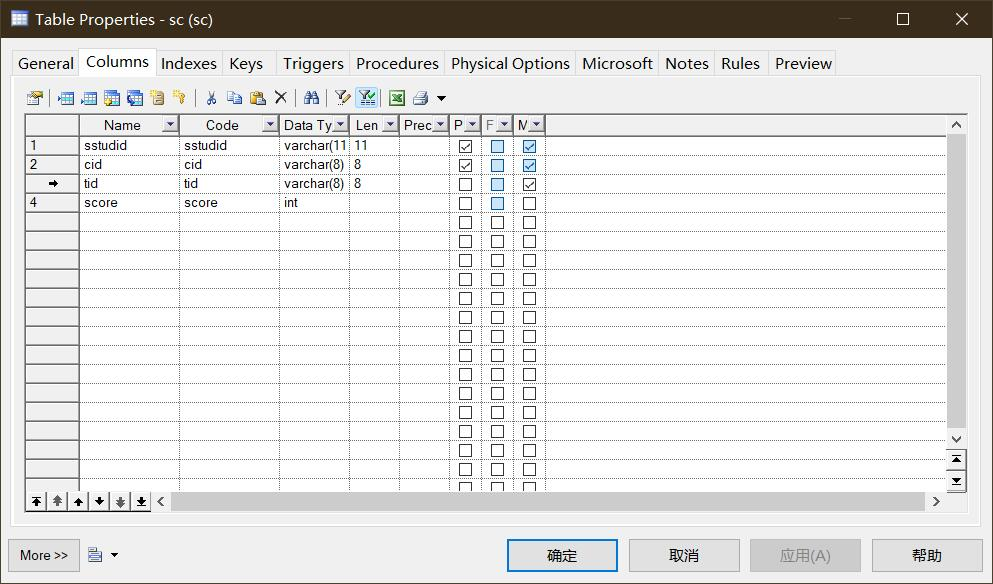
\includegraphics[width=0.8\linewidth]{sc.jpg}
              \caption{sc}
          \end{figure}
          \begin{figure}[!htbp]
              \centering
              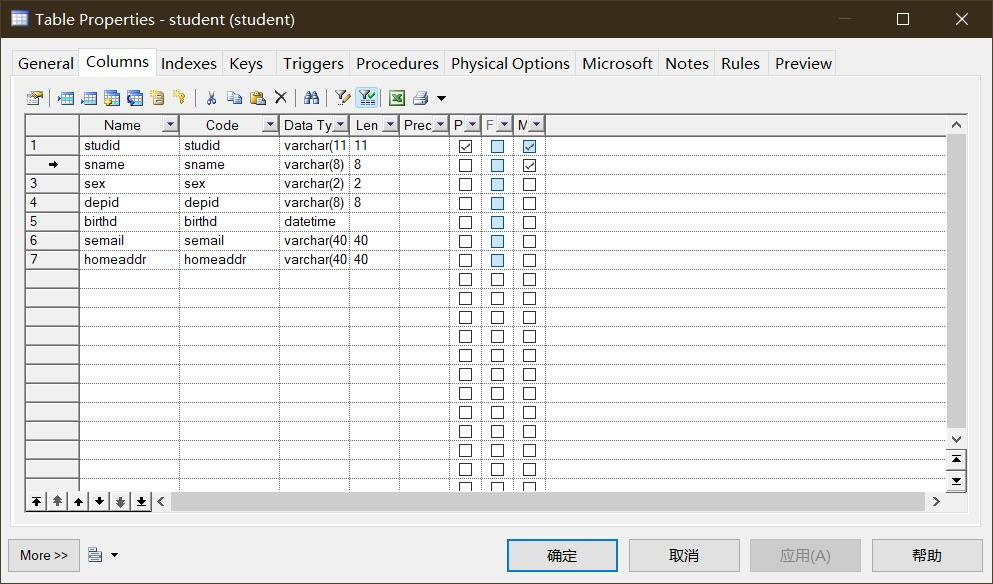
\includegraphics[width=0.8\linewidth]{student.jpg}
              \caption{student}
          \end{figure}
          \newpage
    \item 设置sc表中的score字段以及student表中的sex和semail字段的约束条件。
          \begin{figure}[!htbp]
              \centering
              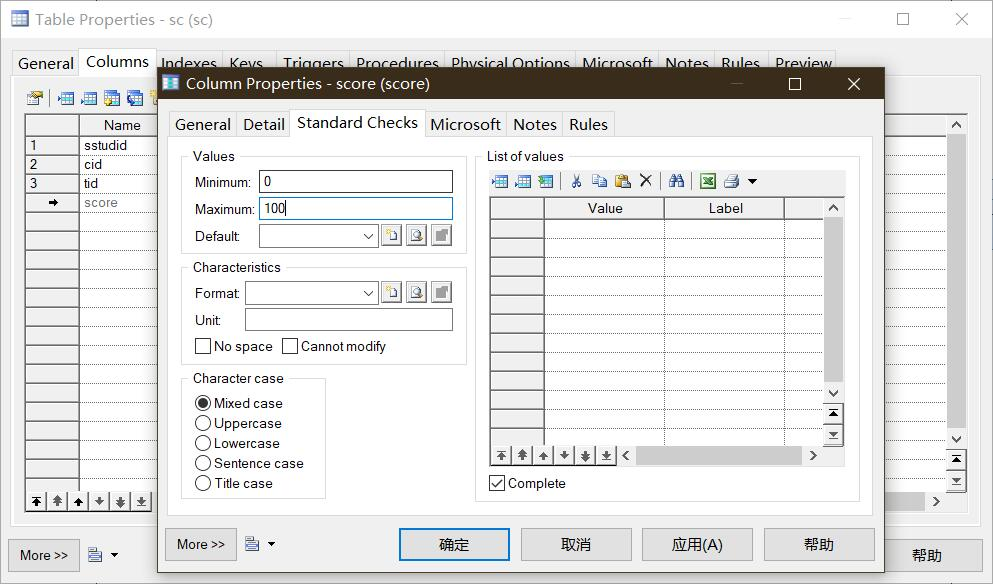
\includegraphics[width=0.8\linewidth]{score.jpg}
              \caption{score约束条件}
          \end{figure}
          \begin{figure}[!htbp]
              \centering
              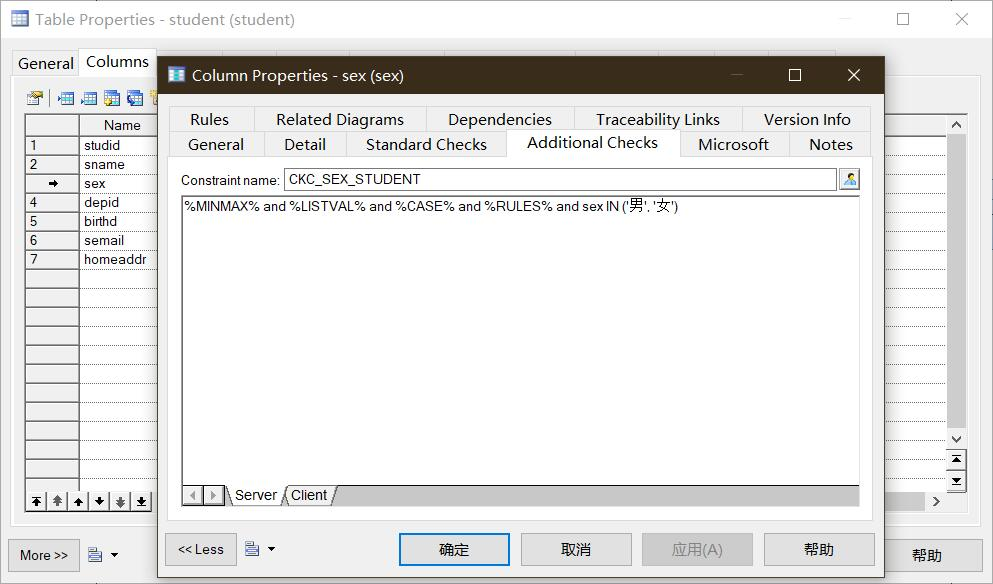
\includegraphics[width=0.8\linewidth]{sex.jpg}
              \caption{sex约束条件}
          \end{figure}
          \begin{figure}[!htbp]
              \centering
              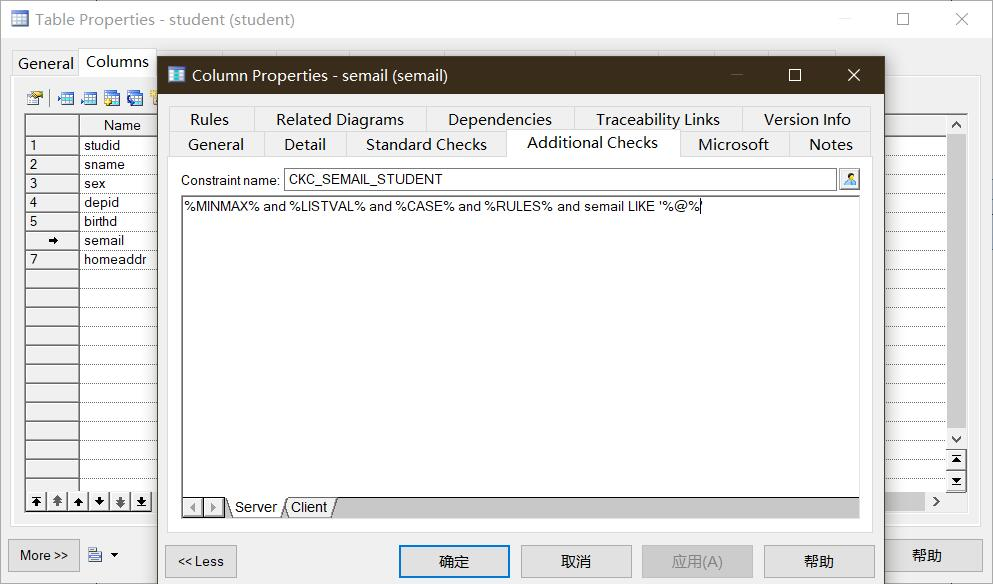
\includegraphics[width=0.8\linewidth]{semail.jpg}
              \caption{semail约束条件}
          \end{figure}
          \newpage
    \item 添加外键。
\end{enumerate}

\subsection{导出数据库的脚本。}

\section{实验数据及结果分析}
最终PDM\_Stud数据库的物理数据模型如下图所示:
\begin{figure}[!htbp]
    \centering
    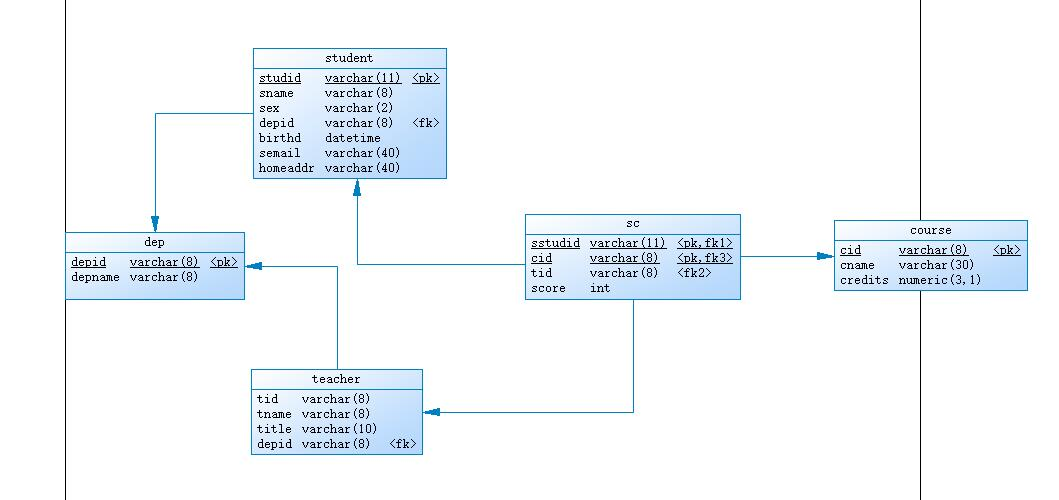
\includegraphics[width=0.8\linewidth]{relation.jpg}
    \caption{PDM\_Stud}
\end{figure}

\section{实验结论、心得体会和改进建议}
掌握数据库建模工具Power Designer设计数据库相关的知识。

\end{document}